\documentclass{article}

\title{\vspace{-2.0cm}Stuff}
\title{ST 599 Project 1 Report}
\author{Wanli Zhang \& Matt Edwards}
\date{21st April 2014}

\usepackage{fullpage}
\usepackage{floatrow} %%http://tex.stackexchange.com/questions/6850/table-and-figure-side-by-side-with-independent-captions
\usepackage{fourier} % uses Adobe font, comment to use latex default font

\usepackage{Sweave}
\begin{document}
%\maketitle %% ==== We may want to do this by hand, to give more room in the rest of the document ====
\Sconcordance{concordance:ProjectReport.tex:ProjectReport.Rnw:%
1 11 1 1 0 89 1}


\begingroup  
  \centering
  \LARGE ST 599 Project 1 Report\\[1em]
  \large Wanli Zhang \& Matt Edwards\par
\endgroup
% uses 2nd answer from here: http://tex.stackexchange.com/questions/29593/shift-title-and-author-text-up

\section{Background $\&$ Questions of Interest}
Our group used the 5-year PUMS data of all states from the American Community Survey, and tackled three questions of interest:

\begin{enumerate}

\item Does prior military service affect, positively or negatively, the maximum amount of schooling received by an individual? %We were curious because in some ways, military service can be viewed as an interruption in the "normal" life flow, one which often starts immediately after high shool or in young adulthood, the times when invidiaals in our culture typically pursue higher education.%
\item Does prior military service affect the salary level of an individual
\item Does prior military service affect whether or not the individual has health insurance coverage? 
\end{enumerate}


\section{Results}
\subsection{Education}
For education, military service does not seem to play a significant role (Figure 2). The median education level is 18 (some college, but no degree) for a vast majority of the state and service level combinations (West Virgina and DC being two notable exceptions.) This analysis is based on The categories for School Level being expressed numerically, and essentially in order (higher numbers mean more education, lower numbers mean less education). However, this is categorical data and some of the levels are functionally equivalent (16 = High School Diploma, 17 = GED) so this graph does not tell the whole story.

\subsection{Wages}
Surprisingly, those who Never Served had a lower median income overall than those who were retired from service, as seen in Figure 1. It is doubtful if there is a statistical difference, as the IQR, as indicated by the error bars, overlap for all categories. 


\begin{figure}[ht!]
\begin{floatrow}
\ffigbox{%
  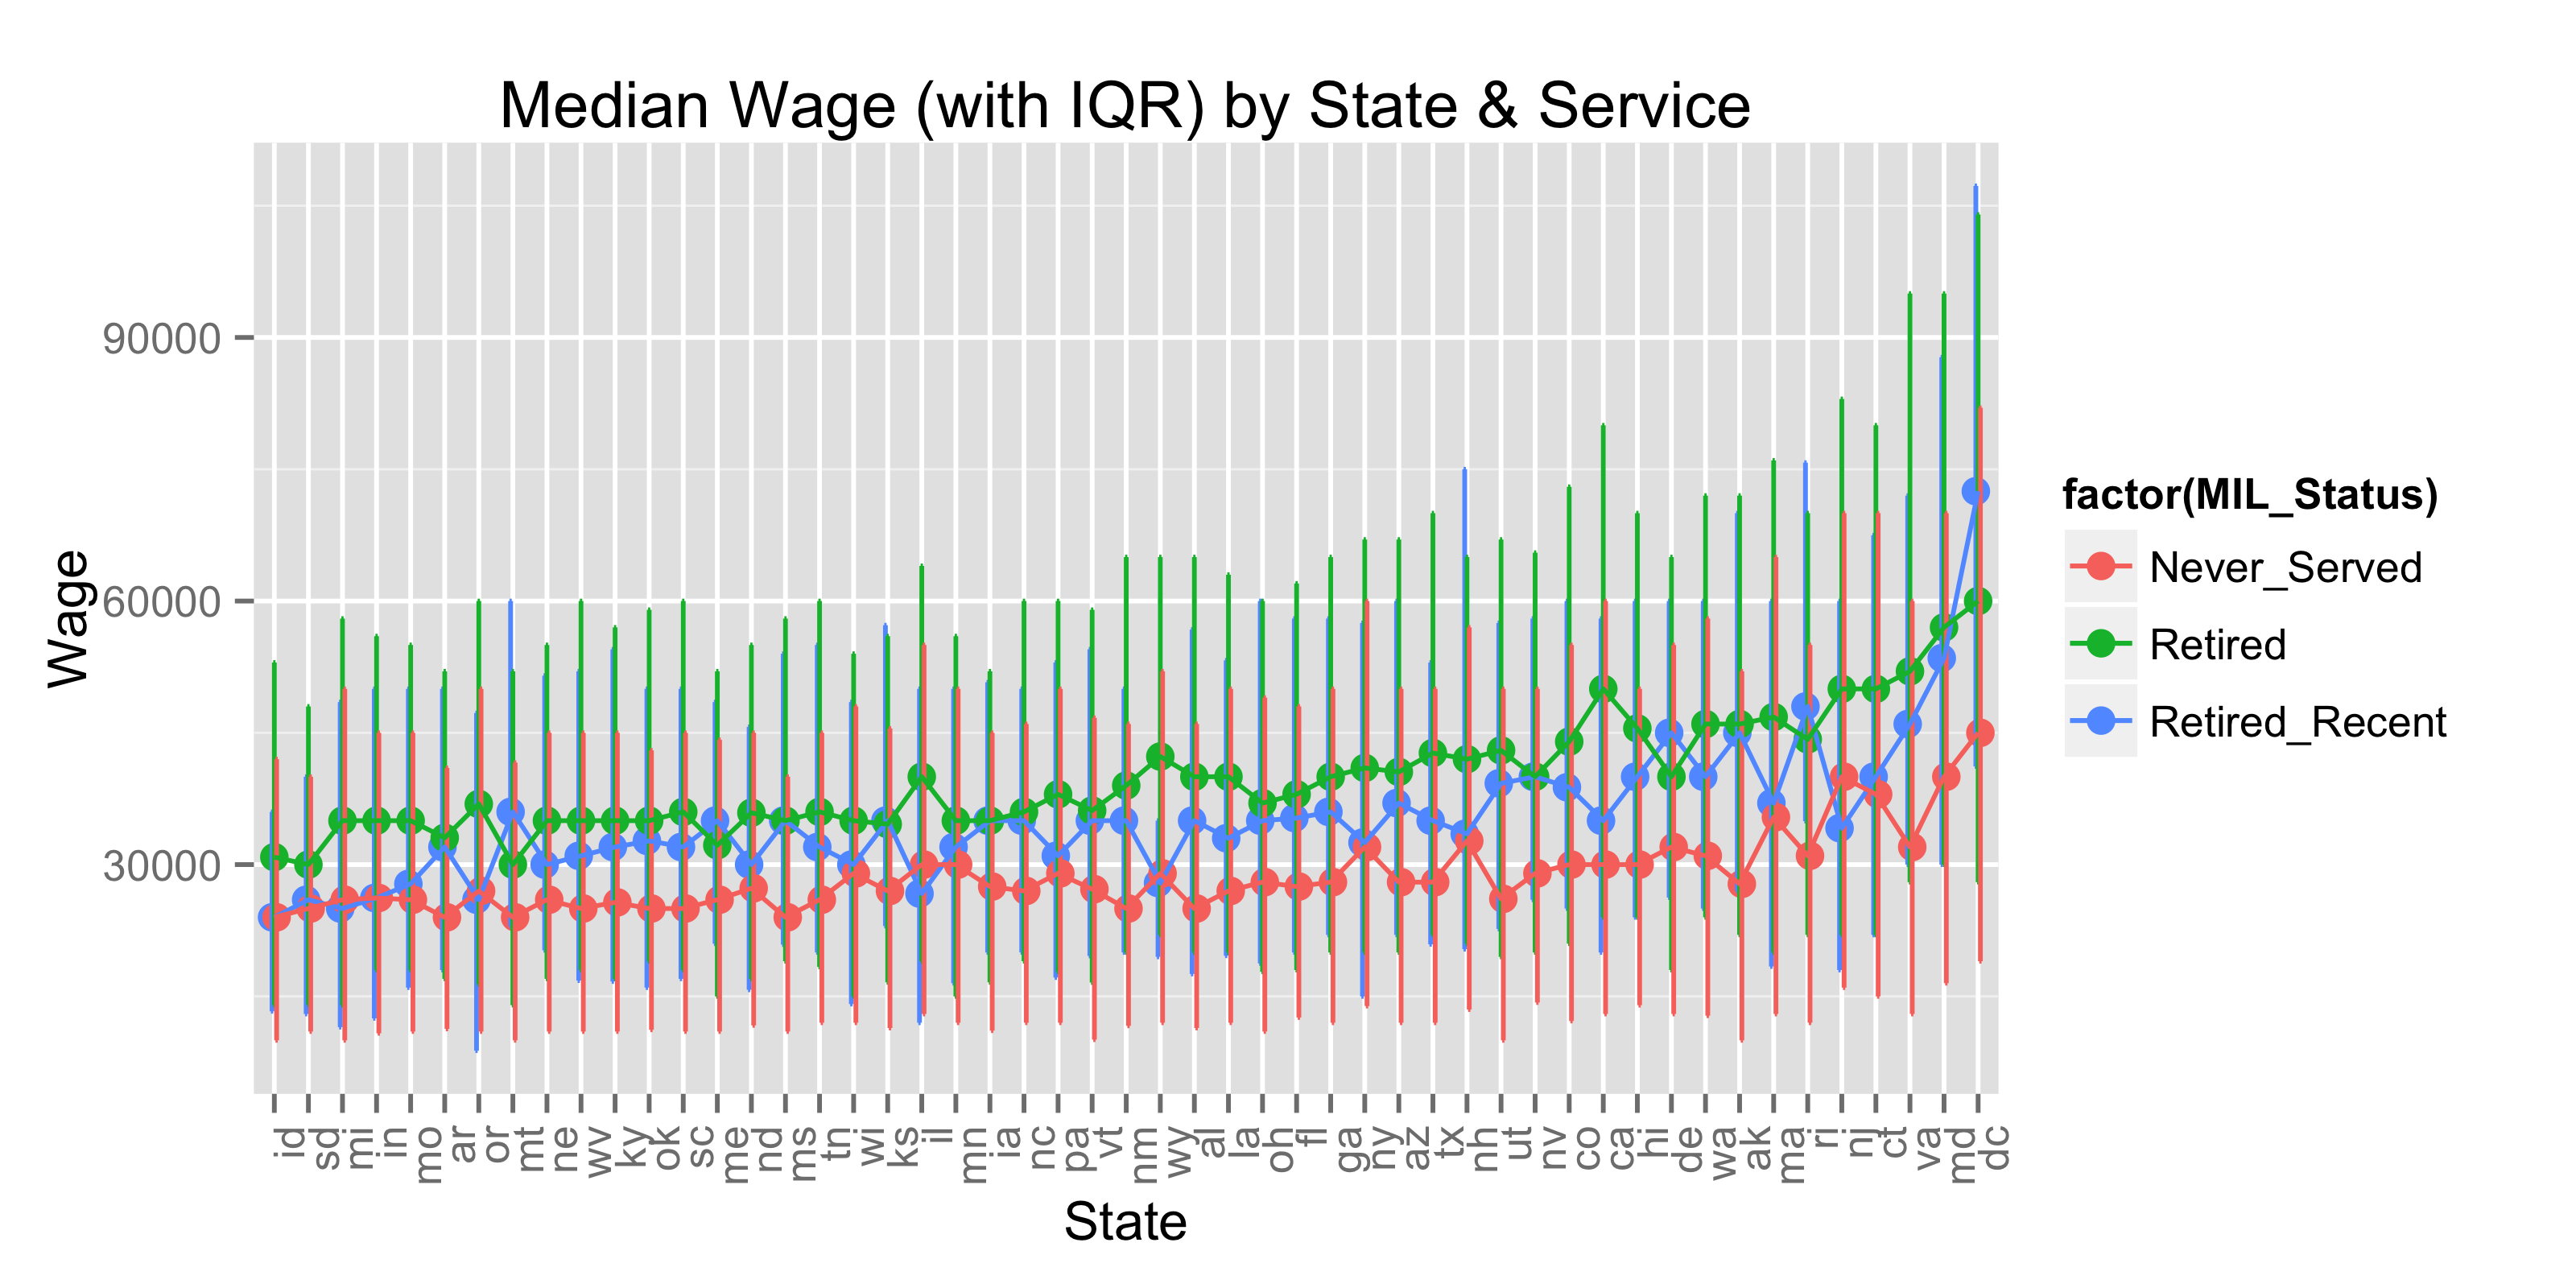
\includegraphics[width=0.5\textwidth]{../Wage_Education/Graphs/Wages}%
}{%
  \caption{Income}%
}
\ffigbox{%
  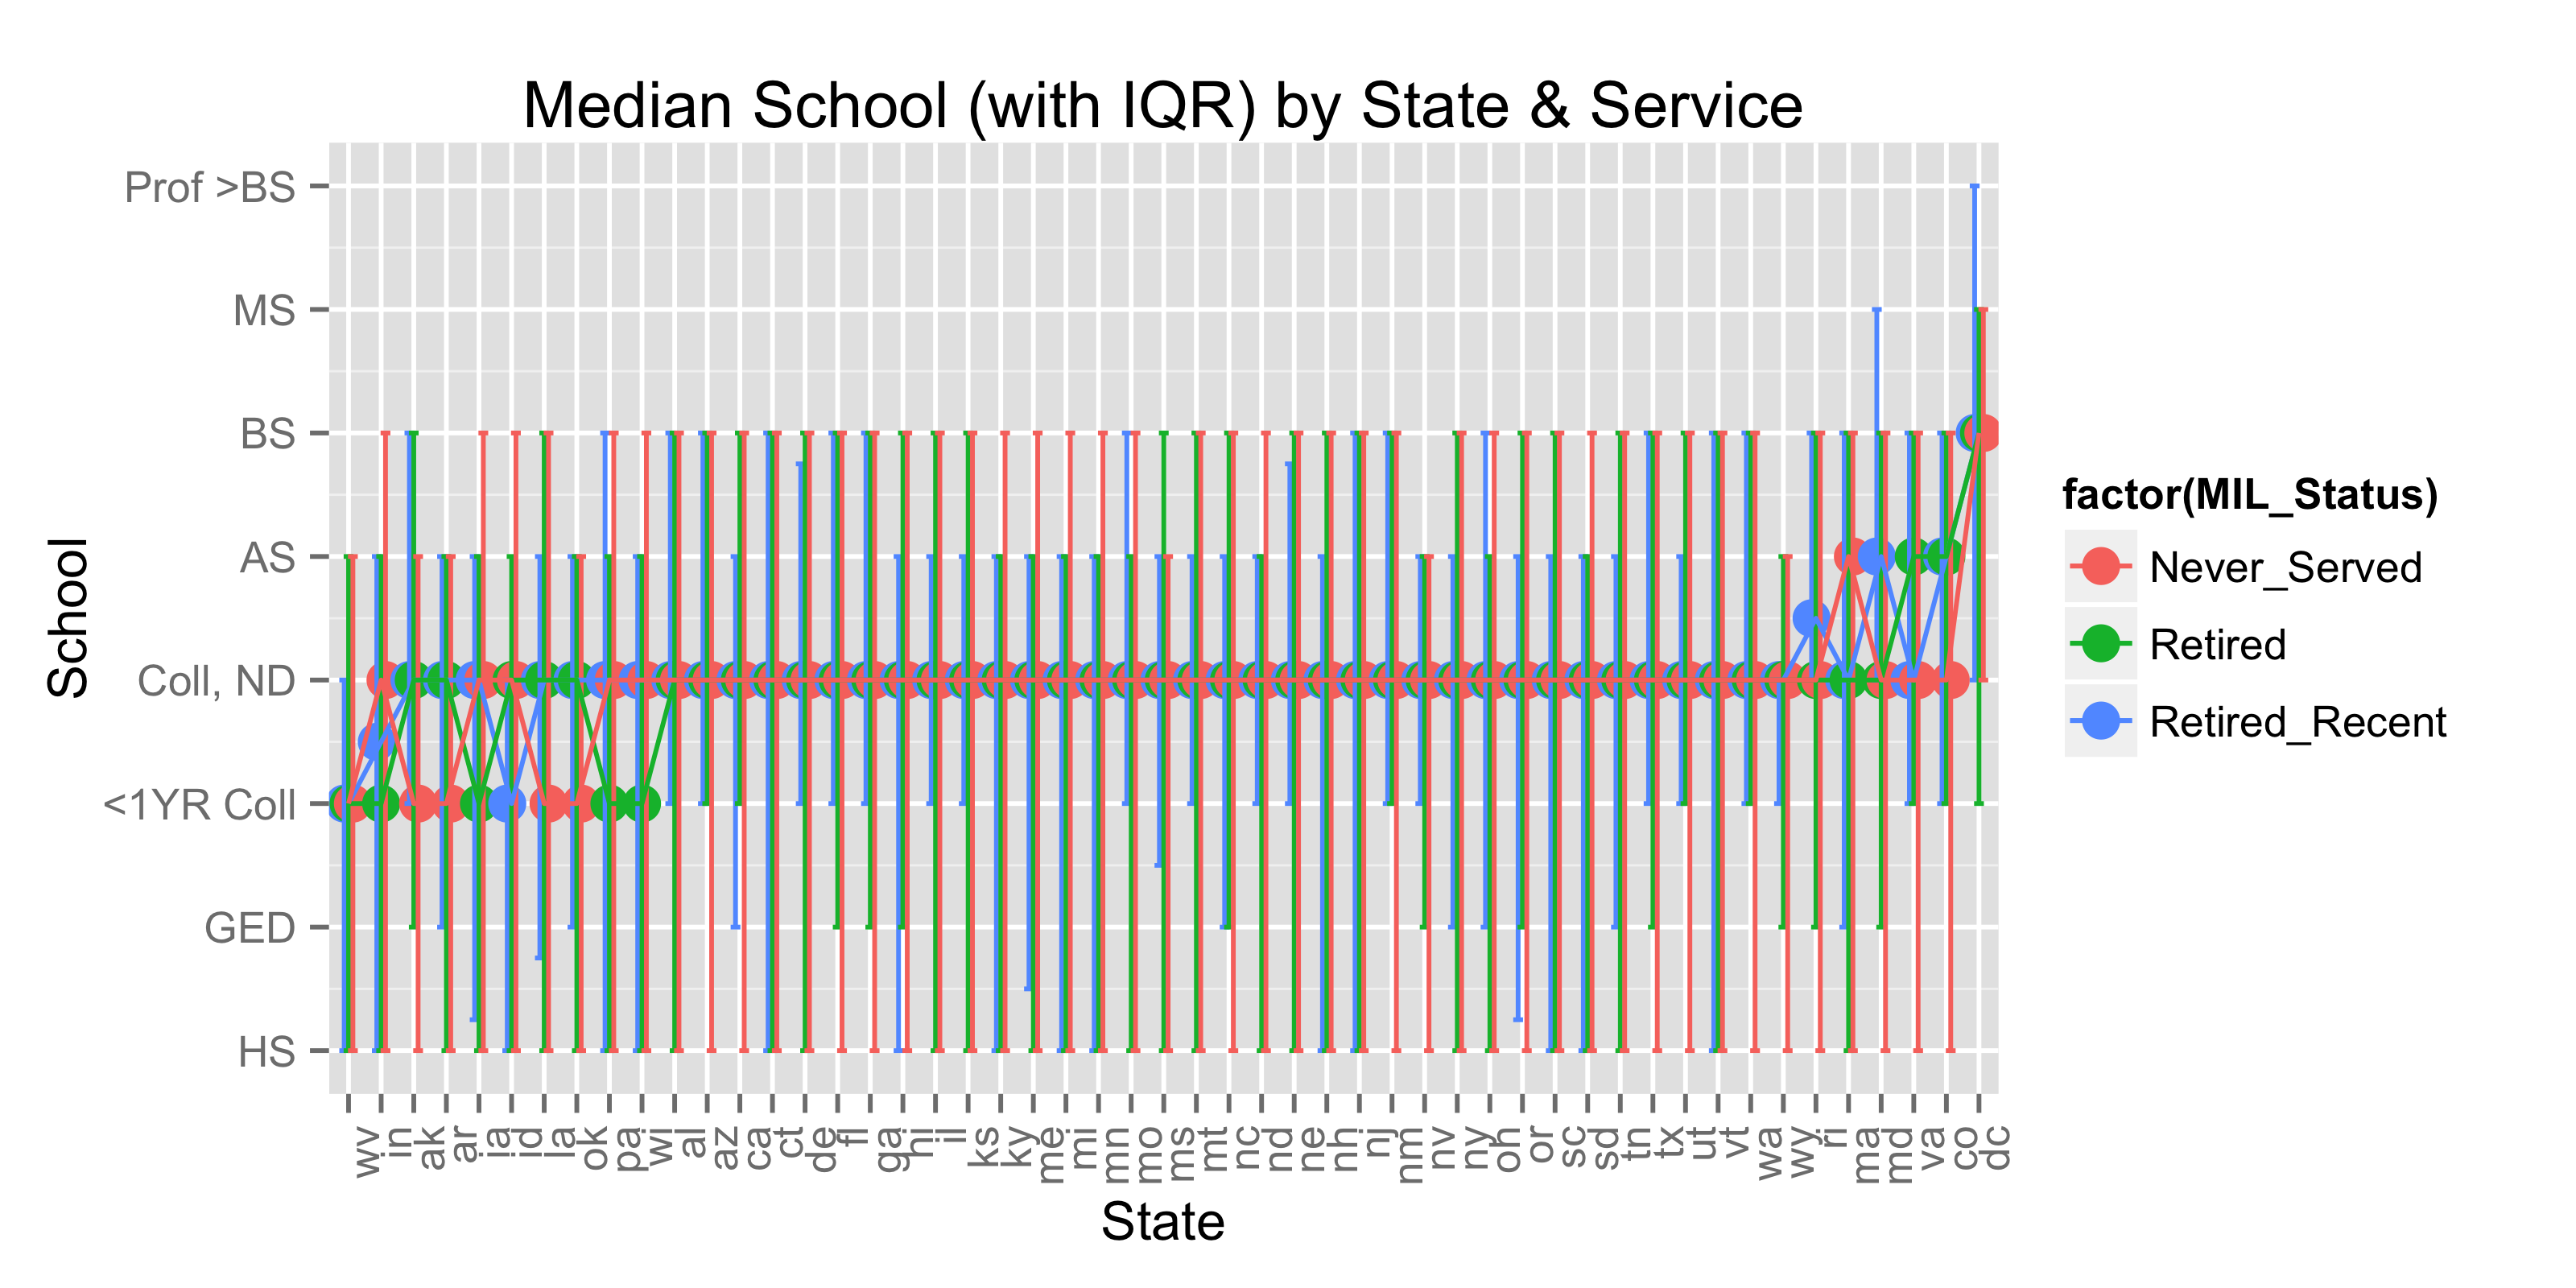
\includegraphics[width=0.5\textwidth]{../Wage_Education/Graphs/School}%
}{%
  \caption{Education}%
}
\end{floatrow}

\end{figure}


%\pagebreak


\subsection{Insurance}
As can be observed in Figure 3, in every state, the health insurance coverage rate for people who have served or are on active duty is greater than that for those who haven't served at all. In fact, as Figure 2 demonstrates, the odds of being covered by health insurance for people who have served are at least two times as those for people who have not. This ratio is largest in California (5.30), and smallest in South Dakota (2.30).

\begin{figure}[ht!]
\begin{floatrow}
\ffigbox{%
  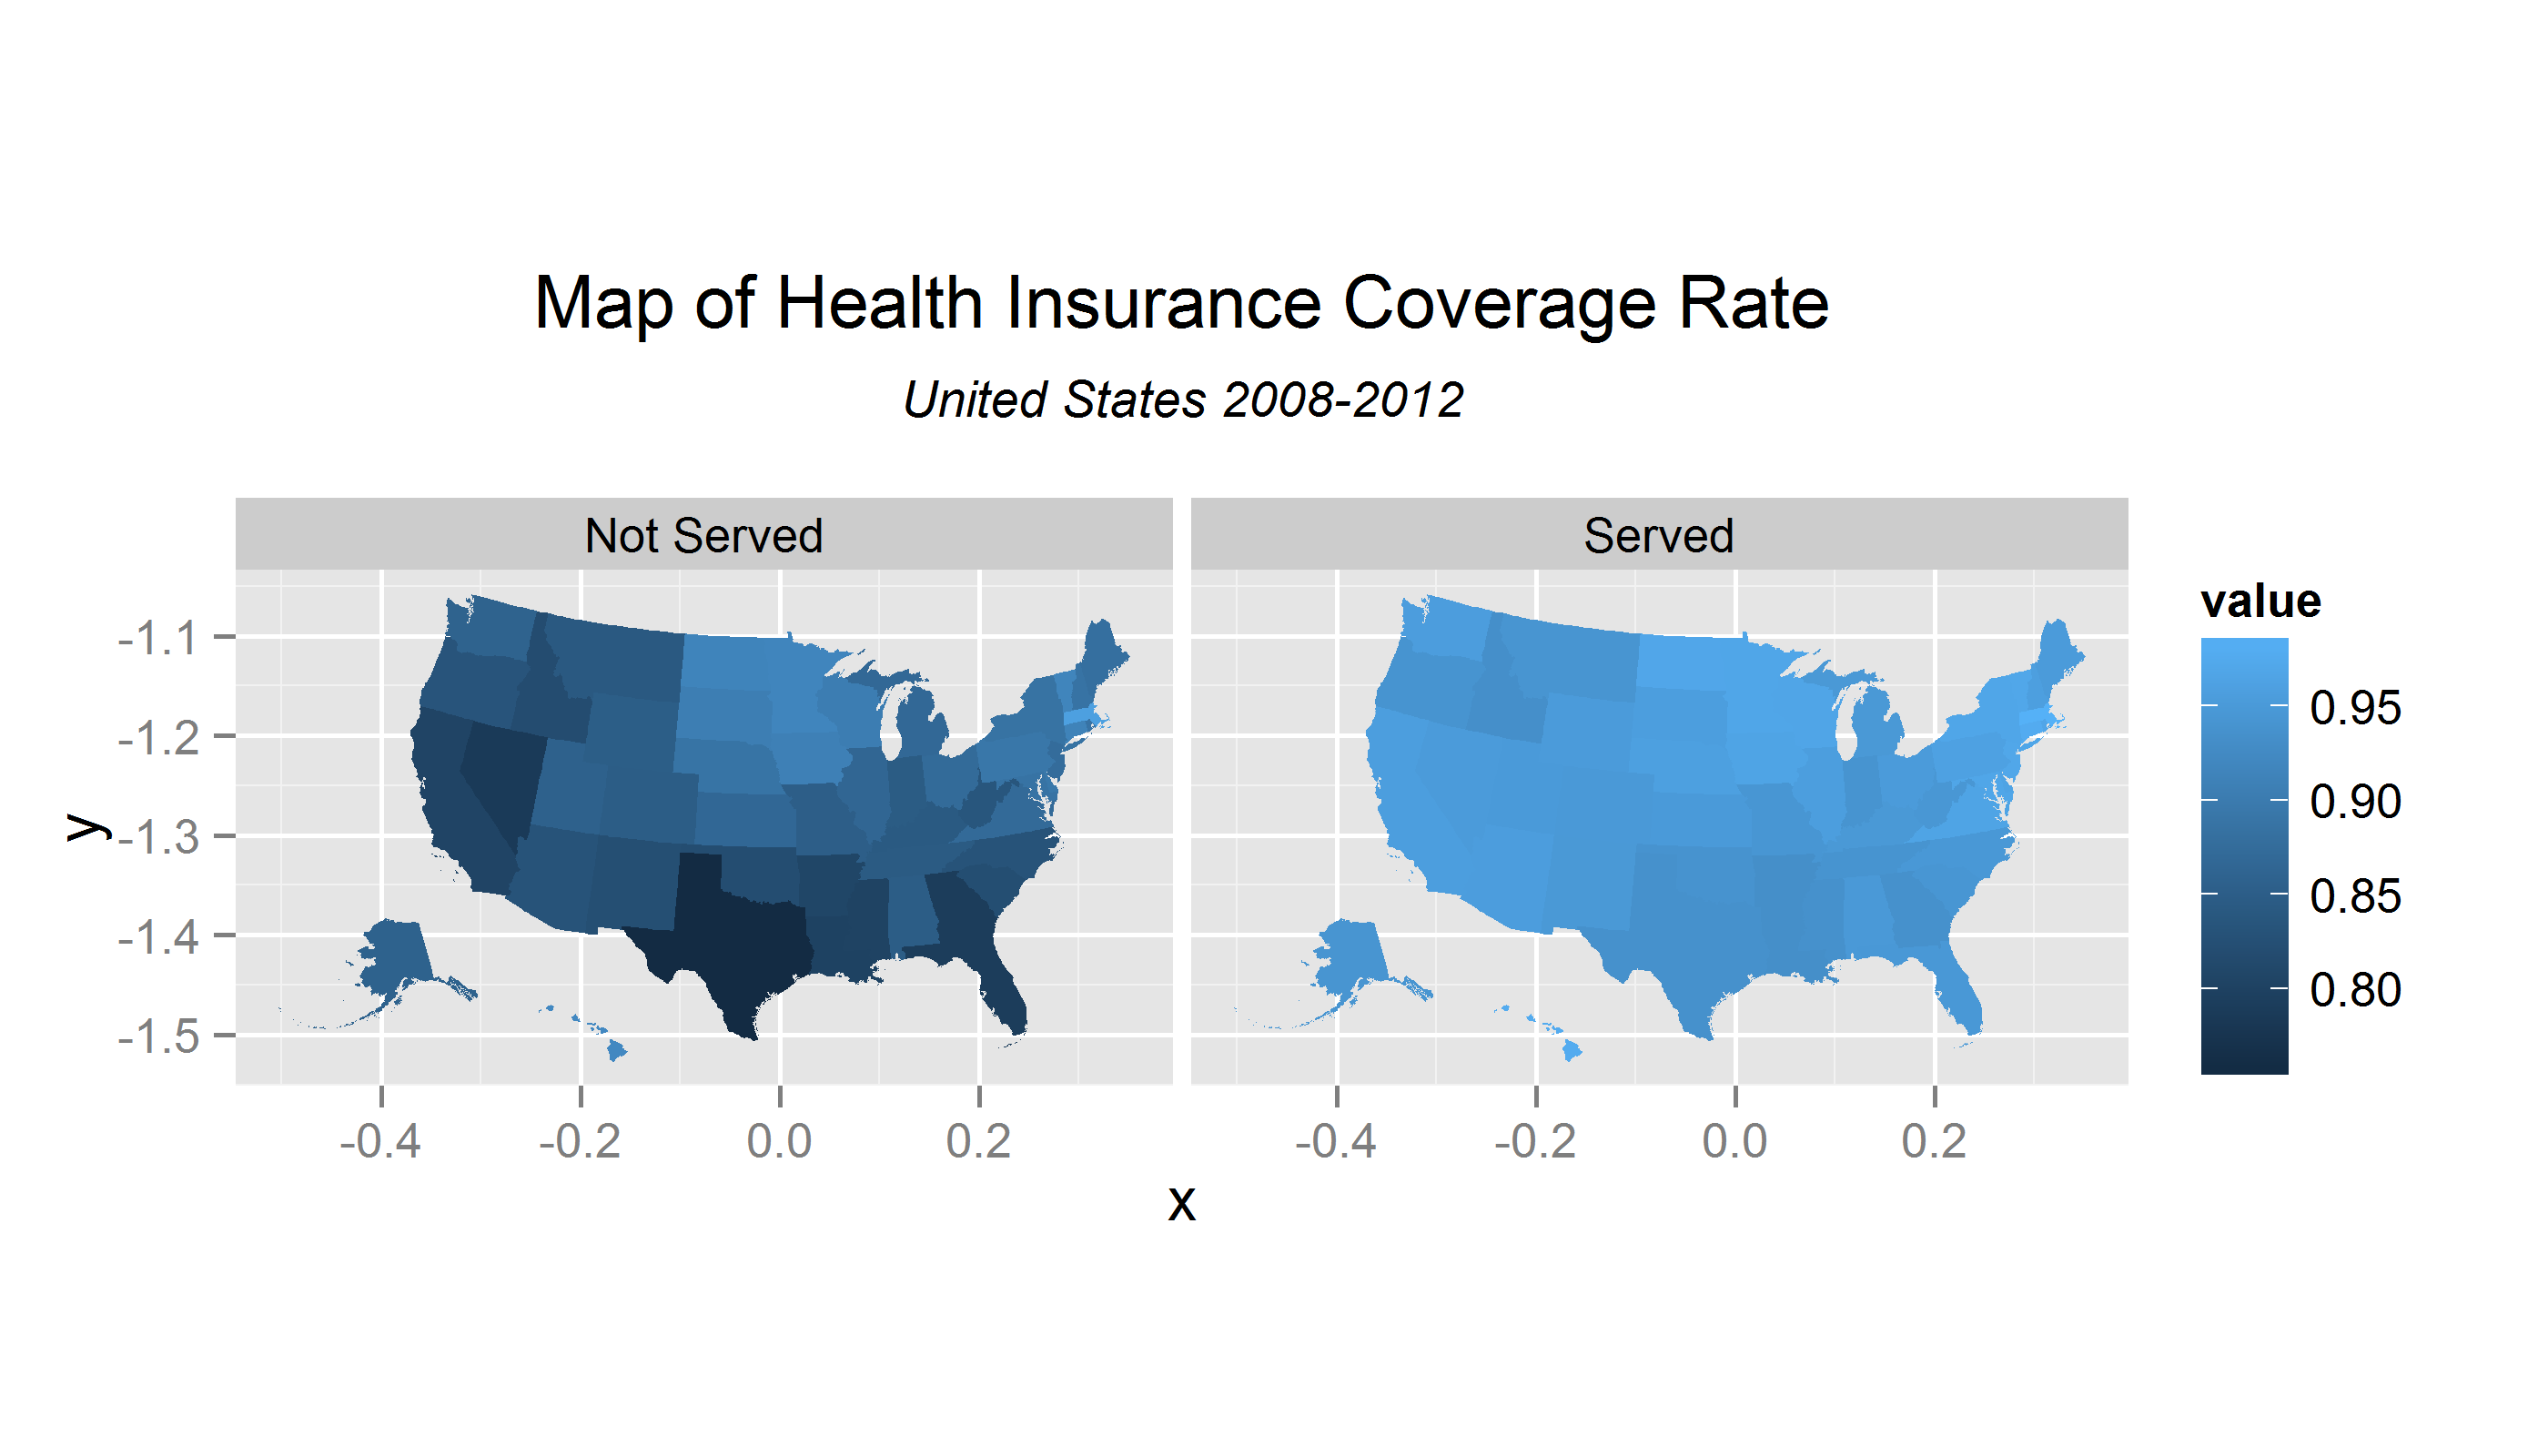
\includegraphics[width=0.5\textwidth]{../Insurance/Graphs/insurance_sbsmap}%
}{%
  \caption{Coverage Rate}%
}
\ffigbox{%
  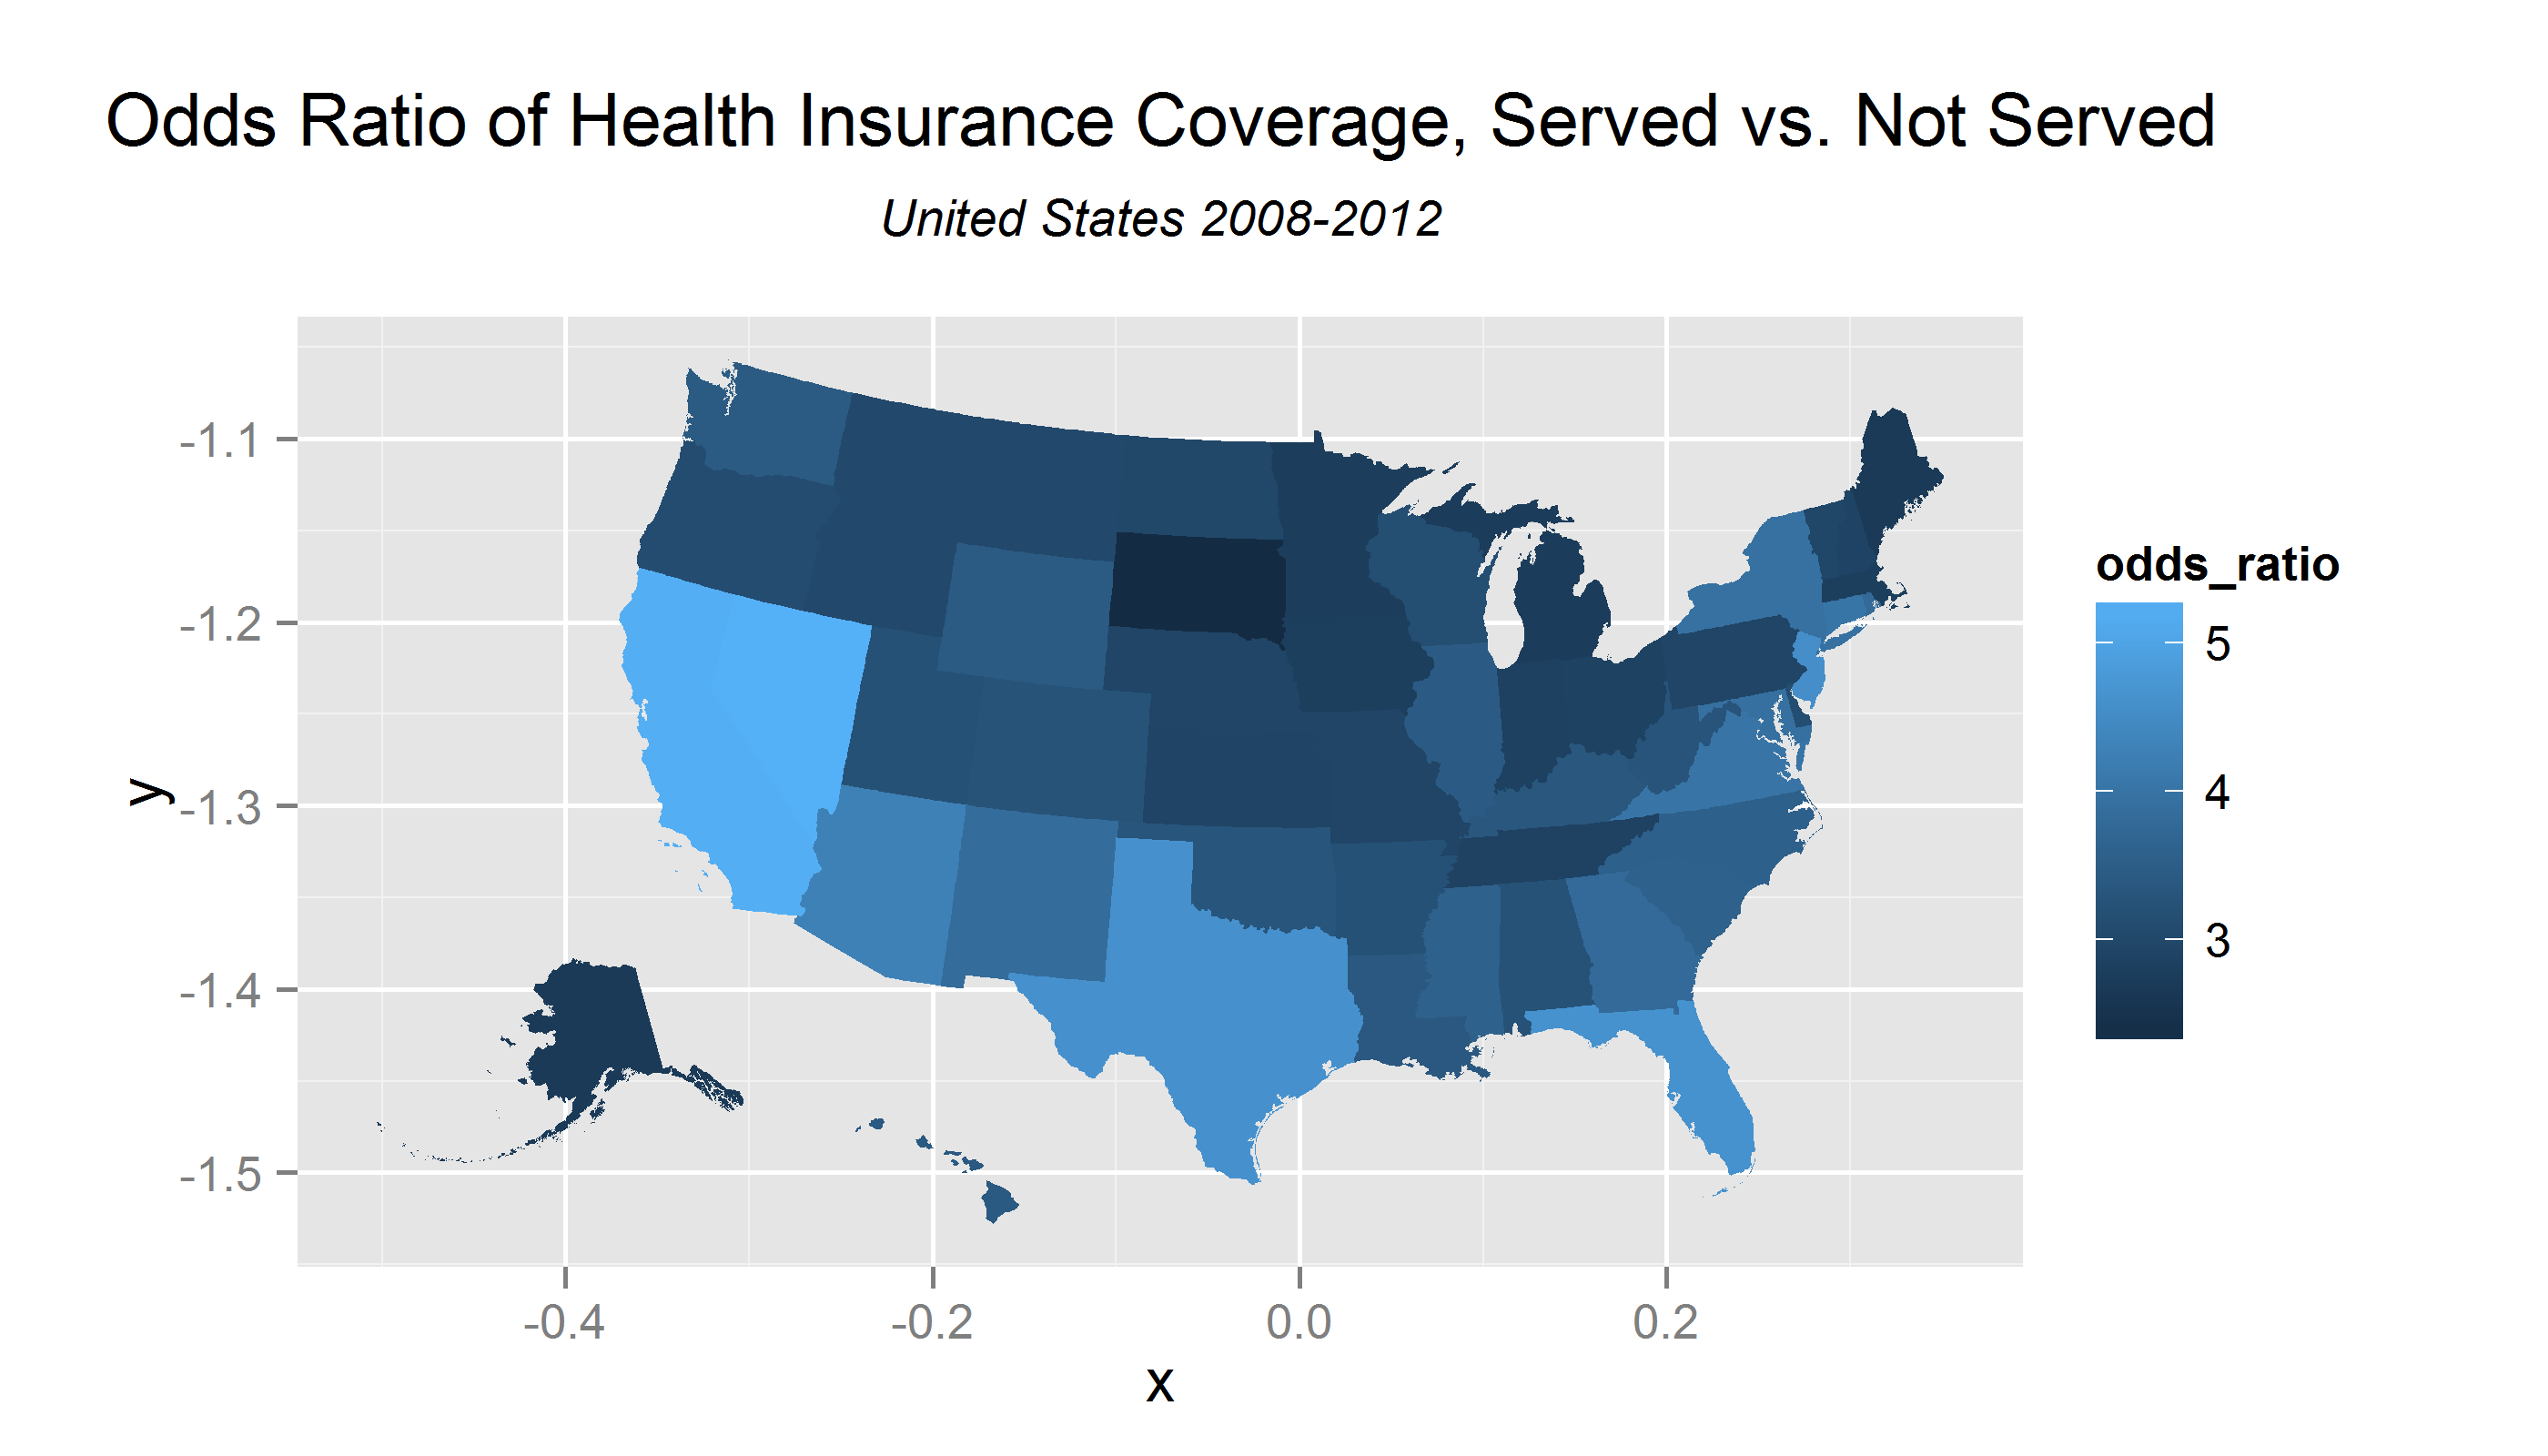
\includegraphics[width=0.5\textwidth]{../Insurance/Graphs/insurance_oddsmap}%
}{%
  \caption{Odds Ratio}%
}
\end{floatrow}

\end{figure}



\section{Obstacles \& Solutions}
For the income question, an obstacle came with the realization that the variable "PINCP" was ALL income sources combined, and the decision to analyze only Wage Income (WAGP.) The WAGP variable is very heavily loaded with zeroes, 46\% of the observations, in fact. Only 10\% of the Total Person Income set were zeroes. The initial question stated "income", but the intent was "Salary", so the data set was trimmed to only Wage values greater than zero. This was a tough decision, because some of those are probably valid zeros (retirees, etc.) while others are not. The question was not necessarily as simple as it started out.\\

One problem we were unable to solve was, with 3 categories on the point chart, it would not settle on one of them to order by. They were overall in order, but no individual category was strictly in order.\\

Another problem came up when we attempted to use odds ratio to describe insruance coverage. Eventually, we decided to further reduce the variable "MIL" to two categories: Served and Not Served.


\section{Future Work}
As noted in the Obstacles section, there is work to be done in the income area. It would be useful to break down the income by the 8 sub-categories that make up Total Person Income (PINCP) and analyze those as they related to military service. How many individuals have other sources of income that contribute more than a Salary? Is there a difference in these levels between prior-service and no-service individuals?\\

One breakdown that would be applied to all three questions is the breakdown of time out of service. There is more granularity available for the timeframe of service (Iraq War, Korean War, Vietnam War, etc.) Breaking the results down by these categories could be informative.\\ 

For the education question, it would be useful to turn the question around, and look at if the proportion of those receiving higher education degrees (BS, MS, PhD) is the same based on prior military service.\\

Finally, we could break down insurance into different types, and it would be interesting to observe which type of insurance is the most popular in each state, among people who either have served or have not.


\end{document}
